\section{Appendix}

\begin{table}[h!]
    \caption{Example of the SLOW5 file format in the ASCII encoding.\label{tab:slow5}}
    \begin{tabular}{|*{7}{l}|}
        \hline
        \multicolumn{7}{|l|}{\#\#file\_format=slow5v0.1} \\
        \#read\_id & n\_samples & digitisation & offset & range & sample\_rate & raw\_signal \\
            \textit{id-0} & 6028 & 8192.0 & 3.0 & 1467.6 & 4000.0 & $1373,712,738,715,716,\dots$ \\
                    \textit{id-1} & 59676 & 8192.0 & 23.0 & 1467.6 & 4000.0 & $1039,588,588,593,586,\dots$ \\
                            \; \vdots & \; \vdots & \;\; \vdots & \; \vdots & \;\; \vdots & \;\; \vdots & \hspace{1cm} \vdots \\
                                    \textit{id-$N$} & 45690 & 8192.0 & 5.0 & 1467.6 & 4000.0 & $1255,773,617,574,568,\dots$ \\

        \hline
    \end{tabular}
\end{table}

\begin{figure}[h!]
	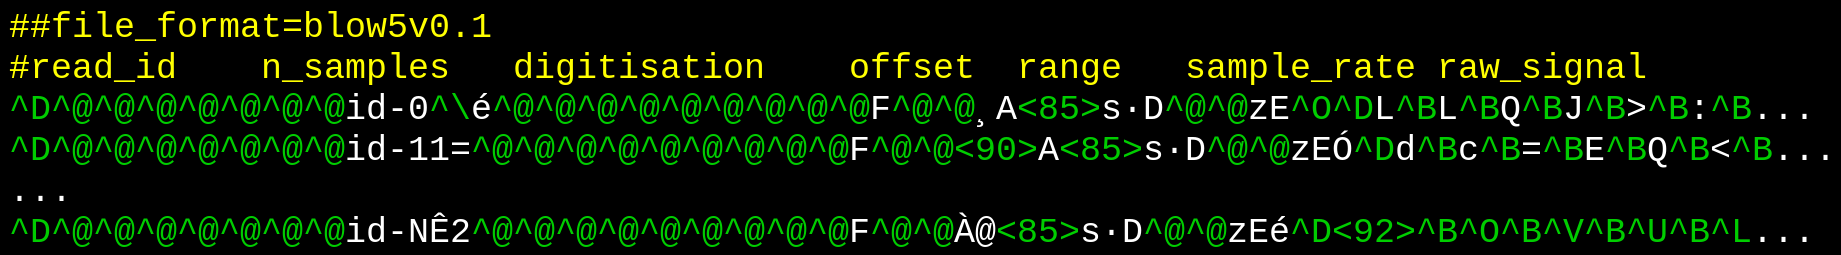
\includegraphics[width=1.5\linewidth]{blow5_nonum.png}
    \caption{Binary encoding of the example SLOW5 file shown in table \ref{tab:slow5}. Note: newline characters between the header and each read have been added for readability and `\dots' indicates where more information is not displayed.}
	\label{tab:blow5}
\end{figure}

\begin{figure}[h!]
	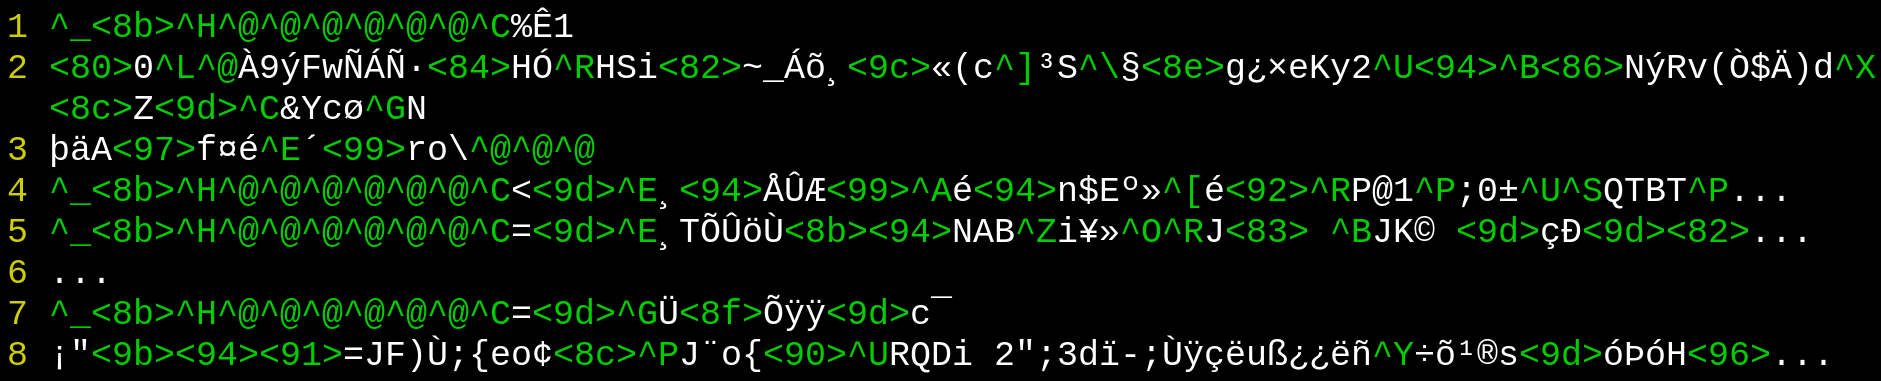
\includegraphics[width=1.5\linewidth]{blow5gz_new.png}
    \caption{Compressed binary encoding of the example SLOW5 file shown in table \ref{tab:slow5}. The header found in figure \ref{tab:blow5} is compressed in lines 1, 2 and 3. Whilst the compressed reads corresponding to read IDs `\textit{id-0}', `\textit{id-1}' and `\textit{id-N}' are found in lines 4, 5 and 7/8 respectively. Note: newline characters between the header and each read have been added for readability and `\dots' indicates where more information is not displayed.}
	\label{tab:blow5gz}
\end{figure}
